\scanpage{151}\mspage{6}
\unsure{groupe|groupes} \unsure{formel|formels} est concentré en les groupes formels commutatifs, découvert semble-t-il par Dieudonné \dots). La question que je voudrais soulever est la généralisation aux groupes dans $(n\text{-cat})$, on s'attend à trouver des complexes de chaines non comm
\diagram{\begin{tikzcd}[ampersand replacement=\&,column sep=small]
L_n\arrow[r,no head,to path={-- (\tikztotarget) -- ++(0.025,0.055)}] \& L_{n-\unsure{,|1}}\arrow[r,no head,to path={-- (\tikztotarget) -- ++(0.025,0.055)}] \& \ldots\arrow[r,no head,to path={-- (\tikztotarget) -- ++(0.025,0.055)}] \& L_1\arrow[r,no head,to path={-- (\tikztotarget) -- ++(0.025,0.055)}] \& L_0\arrow[r] \& 1
\end{tikzcd}}
avec des structures supplémentaires sans doute du type $\unsure{\Theta|\theta}$, mais lesquelles ? Il est entendu que la signification topologique de ces structures, c'est qu'elles expriment exactement les ``types d'homotopie tronqués en dim $\leq n$'' des groupes topologiques. \inserted{\unsure{mesurant} les types d'hom \unsure{tronqués|tr. \deleted{qués}} en dim $\leq n+1$ des espaces top ponctu\unsure{e|é}s connexes \dots)}
% Guide of the preceding interlinear addition: its left end is before As-tu.
\figure{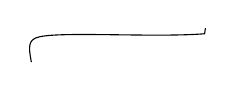
\begin{tikzpicture}\draw (0,0) .. controls (-0.04,0.20) and (-0.04,0.29) .. (0.10,0.32) .. controls (0.38,0.39) and (1.60,0.31) .. (2.20,0.36) -- (2.21,0.43);\end{tikzpicture}}
As-tu des candïdats à proposer ?

\figure{
\begin{tikzpicture}\draw (0,0) .. controls (1.1,0.025) and (1.8,0.025) .. (2.35,-0.025);\end{tikzpicture}}

\unsure{.} Tes réflexions de bidualité \inserted{et d'homologie}, pour formelles qu'elles soient, se rattachent à une foule de développements, dont certains seulement existent, \unsure{dès|dés} \unsure{â|à} présent, et d'autres demanderaient des développements considérables. Voici les réminiscences que m'ouvrent tes \unsure{noïves|naïves} questions :
% Guide of et d'homologie: descending left segment meets the gap after bidualité.
\figure{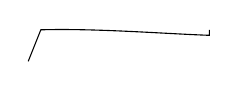
\begin{tikzpicture}\draw (0,0) -- (0.16,0.40) .. controls (0.86,0.42) and (1.73,0.35) .. (2.30,0.33) -- (2.30,0.40);\end{tikzpicture}}
% archive sheet number: 151
